\documentclass{standalone}
\usepackage{tikz}
\usetikzlibrary{patterns, positioning}
\usetikzlibrary{shapes.misc}
\usepackage[outline]{contour}
\contourlength{1.5pt} 
\usepackage[sfdefault]{ClearSans} %% option 'sfdefault' activates Clear Sans as the default text font
\usepackage[T1]{fontenc}

\begin{document}
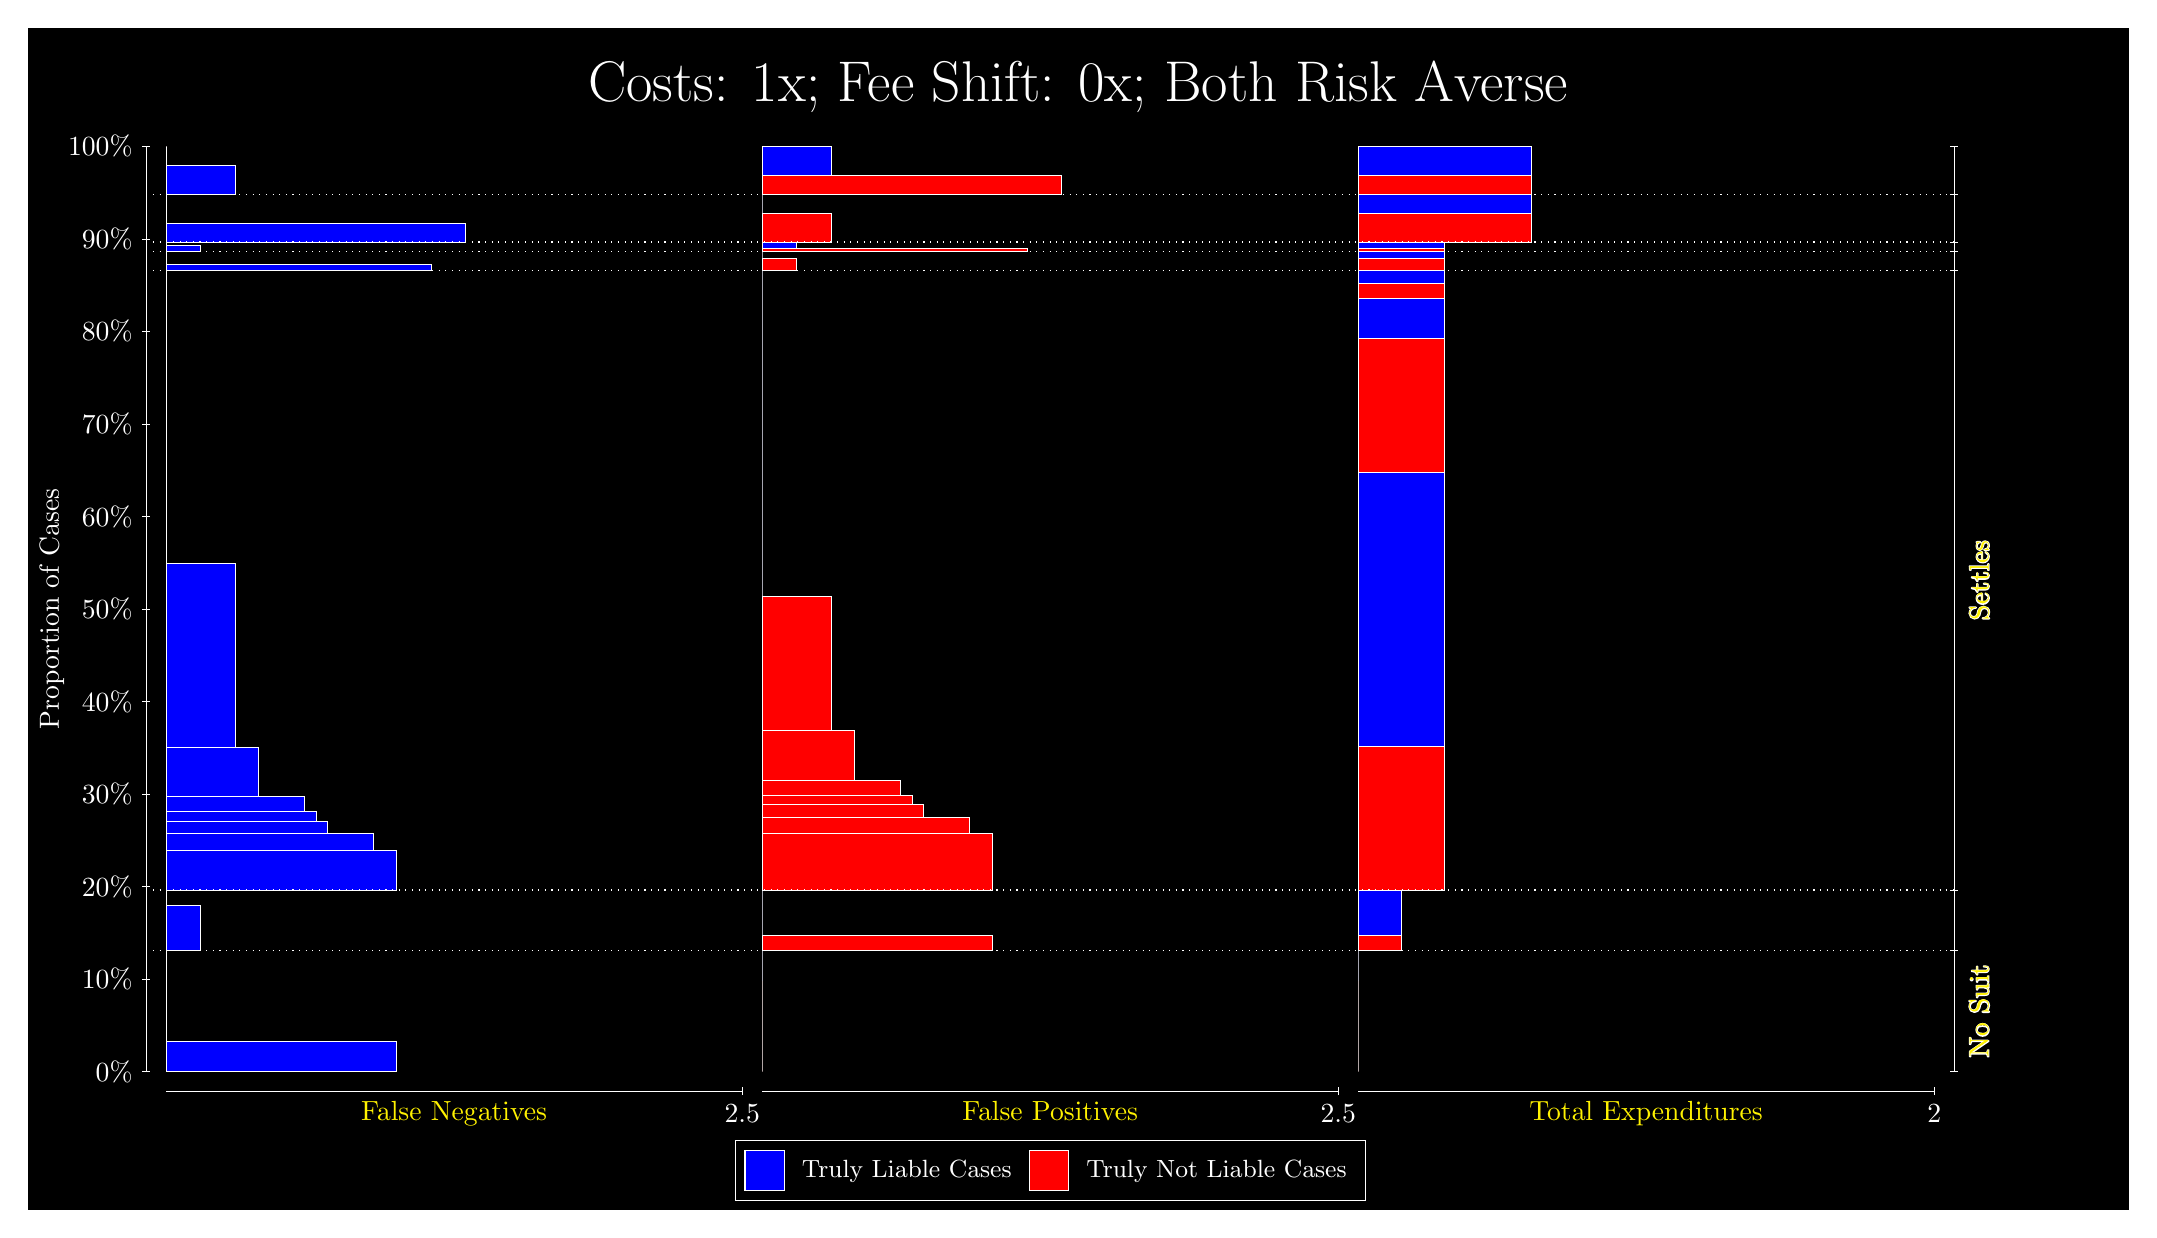
\begin{tikzpicture}
\draw[fill=black] (0,0) rectangle (26.667,15);
\draw[text=white] (0,13.5) rectangle (26.667,15) node[midway] {\huge Costs: 1x; Fee Shift: 0x; Both Risk Averse};
\draw[white, very thin] (1.5,1.75) -- (1.5,13.5);
\node[rotate=90, text=white, anchor=center] at (0.3, 7.625) {Proportion of Cases};
\draw[white, very thin] (1.45,1.75) -- (1.55,1.75);
\node[text=white, anchor=east] at (1.45, 1.75) {0\%};
\draw[white, very thin] (1.45,2.925) -- (1.55,2.925);
\node[text=white, anchor=east] at (1.45, 2.925) {10\%};
\draw[white, very thin] (1.45,4.1) -- (1.55,4.1);
\node[text=white, anchor=east] at (1.45, 4.1) {20\%};
\draw[white, very thin] (1.45,5.275) -- (1.55,5.275);
\node[text=white, anchor=east] at (1.45, 5.275) {30\%};
\draw[white, very thin] (1.45,6.45) -- (1.55,6.45);
\node[text=white, anchor=east] at (1.45, 6.45) {40\%};
\draw[white, very thin] (1.45,7.625) -- (1.55,7.625);
\node[text=white, anchor=east] at (1.45, 7.625) {50\%};
\draw[white, very thin] (1.45,8.8) -- (1.55,8.8);
\node[text=white, anchor=east] at (1.45, 8.8) {60\%};
\draw[white, very thin] (1.45,9.975) -- (1.55,9.975);
\node[text=white, anchor=east] at (1.45, 9.975) {70\%};
\draw[white, very thin] (1.45,11.15) -- (1.55,11.15);
\node[text=white, anchor=east] at (1.45, 11.15) {80\%};
\draw[white, very thin] (1.45,12.325) -- (1.55,12.325);
\node[text=white, anchor=east] at (1.45, 12.325) {90\%};
\draw[white, very thin] (1.45,13.5) -- (1.55,13.5);
\node[text=white, anchor=east] at (1.45, 13.5) {100\%};

\draw[white, very thin] (24.457,1.75) -- (24.457,13.5);
\draw[white, very thin] (24.407,1.75) -- (24.507,1.75);
\node[anchor=west] at (24.407, 1.75) {};
\draw[white, very thin] (24.407,3.2869) -- (24.507,3.2869);
\node[anchor=west] at (24.407, 3.2869) {};
\draw[white, very thin] (24.407,4.0554) -- (24.507,4.0554);
\node[anchor=west] at (24.407, 4.0554) {};
\draw[white, very thin] (24.407,11.924) -- (24.507,11.924);
\node[anchor=west] at (24.407, 11.924) {};
\draw[white, very thin] (24.407,12.165) -- (24.507,12.165);
\node[anchor=west] at (24.407, 12.165) {};
\draw[white, very thin] (24.407,12.285) -- (24.507,12.285);
\node[anchor=west] at (24.407, 12.285) {};
\draw[white, very thin] (24.407,12.893) -- (24.507,12.893);
\node[anchor=west] at (24.407, 12.893) {};
\draw[white, very thin] (24.407,13.5) -- (24.507,13.5);
\node[anchor=west] at (24.407, 13.5) {};

\draw[white, very thin, fill=blue] (1.75,1.75) rectangle (4.6775,2.137);
\draw[white, very thin, fill=red] (1.75,2.137) rectangle (1.75,3.2869);
\draw[white, very thin, fill=blue] (1.75,3.2869) rectangle (2.1891,3.8619);
\draw[white, very thin, fill=red] (1.75,3.8619) rectangle (1.75,4.0554);
\draw[white, very thin, fill=blue] (1.75,4.0554) rectangle (4.6775,4.5662);
\draw[white, very thin, fill=blue] (1.75,4.5662) rectangle (4.3848,4.7755);
\draw[white, very thin, fill=blue] (1.75,4.7755) rectangle (3.7993,4.9336);
\draw[white, very thin, fill=blue] (1.75,4.9336) rectangle (3.6529,5.0498);
\draw[white, very thin, fill=blue] (1.75,5.0498) rectangle (3.5065,5.2448);
\draw[white, very thin, fill=blue] (1.75,5.2448) rectangle (2.921,5.8723);
\draw[white, very thin, fill=blue] (1.75,5.8723) rectangle (2.6283,8.1987);
\draw[white, very thin, fill=red] (1.75,8.1987) rectangle (1.75,11.924);
\draw[white, very thin, fill=blue] (1.75,11.924) rectangle (5.1167,12.008);
\draw[white, very thin, fill=red] (1.75,12.008) rectangle (1.75,12.165);
\draw[white, very thin, fill=blue] (1.75,12.165) rectangle (2.1891,12.243);
\draw[white, very thin, fill=red] (1.75,12.243) rectangle (1.75,12.285);
\draw[white, very thin, fill=blue] (1.75,12.285) rectangle (5.5558,12.527);
\draw[white, very thin, fill=red] (1.75,12.527) rectangle (1.75,12.893);
\draw[white, very thin, fill=blue] (1.75,12.893) rectangle (2.6283,13.258);
\draw[white, very thin, fill=red] (1.75,13.258) rectangle (1.75,13.5);
\draw[white, very thin, fill=red] (9.3189,1.75) rectangle (9.3189,2.8999);
\draw[white, very thin, fill=blue] (9.3189,2.8999) rectangle (9.3189,3.2869);
\draw[white, very thin, fill=red] (9.3189,3.2869) rectangle (12.246,3.4804);
\draw[white, very thin, fill=blue] (9.3189,3.4804) rectangle (9.3189,4.0554);
\draw[white, very thin, fill=red] (9.3189,4.0554) rectangle (12.246,4.7755);
\draw[white, very thin, fill=red] (9.3189,4.7755) rectangle (11.954,4.9848);
\draw[white, very thin, fill=red] (9.3189,4.9848) rectangle (11.368,5.1429);
\draw[white, very thin, fill=red] (9.3189,5.1429) rectangle (11.222,5.2591);
\draw[white, very thin, fill=red] (9.3189,5.2591) rectangle (11.075,5.454);
\draw[white, very thin, fill=red] (9.3189,5.454) rectangle (10.49,6.0816);
\draw[white, very thin, fill=red] (9.3189,6.0816) rectangle (10.197,7.7806);
\draw[white, very thin, fill=blue] (9.3189,7.7806) rectangle (9.3189,11.924);
\draw[white, very thin, fill=red] (9.3189,11.924) rectangle (9.758,12.081);
\draw[white, very thin, fill=blue] (9.3189,12.081) rectangle (9.3189,12.165);
\draw[white, very thin, fill=red] (9.3189,12.165) rectangle (12.686,12.207);
\draw[white, very thin, fill=blue] (9.3189,12.207) rectangle (9.758,12.285);
\draw[white, very thin, fill=red] (9.3189,12.285) rectangle (10.197,12.651);
\draw[white, very thin, fill=blue] (9.3189,12.651) rectangle (9.3189,12.893);
\draw[white, very thin, fill=red] (9.3189,12.893) rectangle (13.125,13.135);
\draw[white, very thin, fill=blue] (9.3189,13.135) rectangle (10.197,13.5);
\draw[white, very thin, fill=red] (16.888,1.75) rectangle (16.888,2.8999);
\draw[white, very thin, fill=blue] (16.888,2.8999) rectangle (16.888,3.2869);
\draw[white, very thin, fill=red] (16.888,3.2869) rectangle (17.437,3.4804);
\draw[white, very thin, fill=blue] (16.888,3.4804) rectangle (17.437,4.0554);
\draw[white, very thin, fill=red] (16.888,4.0554) rectangle (17.986,5.8867);
\draw[white, very thin, fill=blue] (16.888,5.8867) rectangle (17.986,9.3612);
\draw[white, very thin, fill=red] (16.888,9.3612) rectangle (17.986,11.06);
\draw[white, very thin, fill=blue] (16.888,11.06) rectangle (17.986,11.571);
\draw[white, very thin, fill=red] (16.888,11.571) rectangle (17.986,11.766);
\draw[white, very thin, fill=blue] (16.888,11.766) rectangle (17.986,11.924);
\draw[white, very thin, fill=red] (16.888,11.924) rectangle (17.986,12.081);
\draw[white, very thin, fill=blue] (16.888,12.081) rectangle (17.986,12.165);
\draw[white, very thin, fill=red] (16.888,12.165) rectangle (17.986,12.207);
\draw[white, very thin, fill=blue] (16.888,12.207) rectangle (17.986,12.285);
\draw[white, very thin, fill=red] (16.888,12.285) rectangle (19.083,12.651);
\draw[white, very thin, fill=blue] (16.888,12.651) rectangle (19.083,12.893);
\draw[white, very thin, fill=red] (16.888,12.893) rectangle (19.083,13.135);
\draw[white, very thin, fill=blue] (16.888,13.135) rectangle (19.083,13.5);
\draw[white, dotted] (1.5,3.2869) -- (24.457,3.2869);
\draw[white, dotted] (1.5,4.0554) -- (24.457,4.0554);
\draw[white, dotted] (1.5,11.924) -- (24.457,11.924);
\draw[white, dotted] (1.5,12.165) -- (24.457,12.165);
\draw[white, dotted] (1.5,12.285) -- (24.457,12.285);
\draw[white, dotted] (1.5,12.893) -- (24.457,12.893);
\draw[white, very thin] (1.75,1.5) -- (9.0689,1.5);
\node[text=yellow, anchor=north] at (5.4094, 1.5) {False Negatives};
\draw[white, very thin] (9.0689,1.45) -- (9.0689,1.55);
\node[text=white, anchor=north] at (9.0689, 1.45) {2.5};

\draw[white, very thin] (9.3189,1.5) -- (16.638,1.5);
\node[text=yellow, anchor=north] at (12.978, 1.5) {False Positives};
\draw[white, very thin] (16.638,1.45) -- (16.638,1.55);
\node[text=white, anchor=north] at (16.638, 1.45) {2.5};

\draw[white, very thin] (16.888,1.5) -- (24.207,1.5);
\node[text=yellow, anchor=north] at (20.547, 1.5) {Total Expenditures};
\draw[white, very thin] (24.207,1.45) -- (24.207,1.55);
\node[text=white, anchor=north] at (24.207, 1.45) {2};

\node[text=yellow, centered, rotate=90] at (24.777, 2.5185) {\contour{white}{No Suit}};

\node[text=yellow, centered, rotate=90] at (24.777, 7.9896) {\contour{white}{Settles}};





\draw (12.978300999999998,1.5) node[draw=none] (baseCoordinate) {};
\begin{scope}[align=center]
        \matrix[scale=0.5, draw=white, below=0.5cm of baseCoordinate, nodes={draw}, column sep=0.1cm]{
            \node[rectangle, draw, minimum width=0.5cm, minimum height=0.5cm, fill=blue] {}; &
            \node[draw=none, font=\small, text=white] (B) {Truly Liable Cases}; &
            \node[rectangle, draw, minimum width=0.5cm, minimum height=0.5cm, fill=red] {}; &
            \node[draw=none, font=\small, text=white] (B) {Truly Not Liable Cases}; \\
            };
\end{scope}

\end{tikzpicture}
\end{document}